% Generated by code/needham.py -- do not edit by hand.
\definecolor{qocA}{rgb}{0.00,0.45,0.70}
\definecolor{qocB}{rgb}{0.90,0.60,0.00}
\definecolor{qocC}{rgb}{0.00,0.62,0.45}
\definecolor{qocD}{rgb}{0.80,0.40,0.00}
\definecolor{qocE}{rgb}{0.80,0.60,0.70}
\definecolor{qocF}{rgb}{0.35,0.70,0.90}
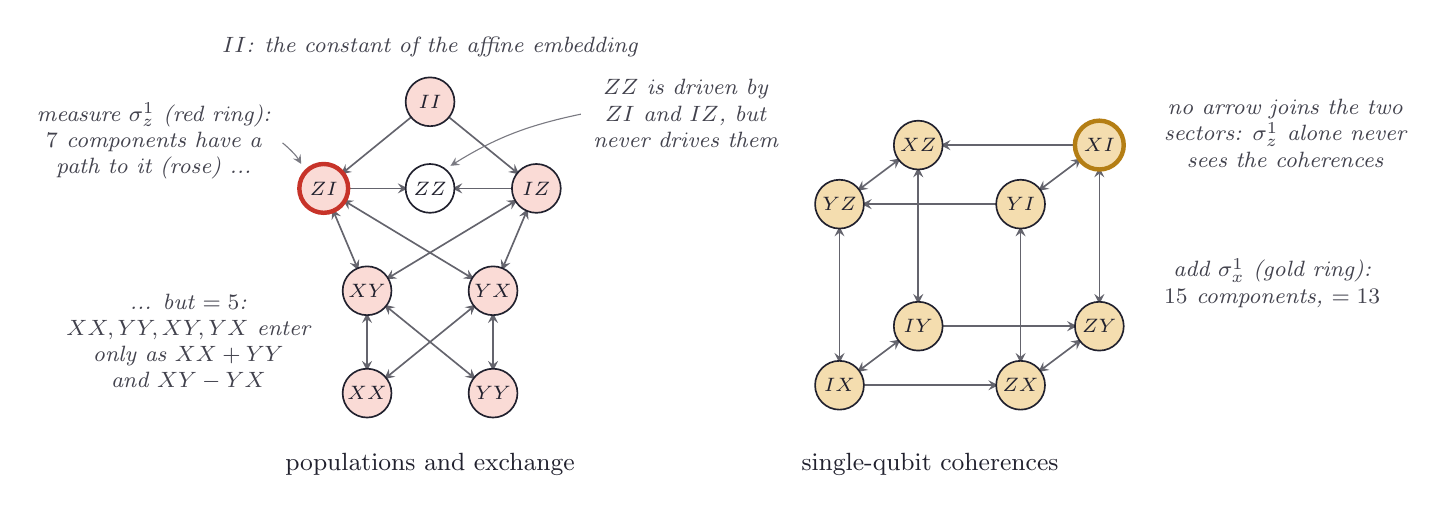
\begin{tikzpicture}[ink/.style={line width=0.9pt, ndInk}, faint/.style={line width=0.4pt, ndInk!35}, dashedink/.style={line width=0.5pt, ndInk!55, dash pattern=on 2.5pt off 2pt}, vec/.style={->, >=stealth, line width=1.2pt}, note/.style={font=\footnotesize\itshape, text=ndInk!85, align=center}, pointer/.style={->, >=stealth, line width=0.4pt, ndInk!60, shorten >=2pt, shorten <=1pt}, dot/.style={circle, fill=ndInk, inner sep=0pt, minimum size=3.4pt}, wash/.style={fill=ndSky, fill opacity=0.55}, every node/.style={text=ndInk}]
\definecolor{ndInk}{rgb}{0.13,0.13,0.18}
\definecolor{ndPaper}{rgb}{0.99,0.96,0.88}
\definecolor{ndSky}{rgb}{0.84,0.91,0.98}
\definecolor{ndRose}{rgb}{0.98,0.86,0.84}
\definecolor{ndBlue}{rgb}{0.13,0.36,0.66}
\definecolor{ndRed}{rgb}{0.78,0.20,0.16}
\definecolor{ndGold}{rgb}{0.88,0.62,0.10}
\definecolor{ndGreen}{rgb}{0.18,0.52,0.30}
\draw[->, >=stealth, line width=0.6pt, ndInk!70, shorten <=8pt, shorten >=8pt] (0.00,2.70) -- (1.35,1.60);
\draw[->, >=stealth, line width=0.6pt, ndInk!70, shorten <=8pt, shorten >=8pt] (0.00,2.70) -- (-1.35,1.60);
\draw[<->, >=stealth, line width=0.6pt, ndInk!70, shorten <=8pt, shorten >=8pt] (5.20,-0.90) -- (6.20,-0.15);
\draw[<->, >=stealth, line width=0.6pt, ndInk!70, shorten <=8pt, shorten >=8pt] (5.20,-0.90) -- (5.20,1.40);
\draw[->, >=stealth, line width=0.6pt, ndInk!70, shorten <=8pt, shorten >=8pt] (5.20,-0.90) -- (7.50,-0.90);
\draw[<->, >=stealth, line width=0.6pt, ndInk!70, shorten <=8pt, shorten >=8pt] (6.20,-0.15) -- (6.20,2.15);
\draw[->, >=stealth, line width=0.6pt, ndInk!70, shorten <=8pt, shorten >=8pt] (6.20,-0.15) -- (8.50,-0.15);
\draw[<->, >=stealth, line width=0.6pt, ndInk!70, shorten <=8pt, shorten >=8pt] (1.35,1.60) -- (-0.80,0.30);
\draw[<->, >=stealth, line width=0.6pt, ndInk!70, shorten <=8pt, shorten >=8pt] (1.35,1.60) -- (0.80,0.30);
\draw[->, >=stealth, line width=0.6pt, ndInk!70, shorten <=8pt, shorten >=8pt] (1.35,1.60) -- (0.00,1.60);
\draw[->, >=stealth, line width=0.6pt, ndInk!70, shorten <=8pt, shorten >=8pt] (8.50,2.15) -- (6.20,2.15);
\draw[<->, >=stealth, line width=0.6pt, ndInk!70, shorten <=8pt, shorten >=8pt] (8.50,2.15) -- (7.50,1.40);
\draw[<->, >=stealth, line width=0.6pt, ndInk!70, shorten <=8pt, shorten >=8pt] (8.50,2.15) -- (8.50,-0.15);
\draw[<->, >=stealth, line width=0.6pt, ndInk!70, shorten <=8pt, shorten >=8pt] (-0.80,-1.00) -- (-0.80,0.30);
\draw[<->, >=stealth, line width=0.6pt, ndInk!70, shorten <=8pt, shorten >=8pt] (-0.80,-1.00) -- (0.80,0.30);
\draw[<->, >=stealth, line width=0.6pt, ndInk!70, shorten <=8pt, shorten >=8pt] (-0.80,0.30) -- (0.80,-1.00);
\draw[<->, >=stealth, line width=0.6pt, ndInk!70, shorten <=8pt, shorten >=8pt] (-0.80,0.30) -- (-1.35,1.60);
\draw[<->, >=stealth, line width=0.6pt, ndInk!70, shorten <=8pt, shorten >=8pt] (6.20,2.15) -- (5.20,1.40);
\draw[->, >=stealth, line width=0.6pt, ndInk!70, shorten <=8pt, shorten >=8pt] (7.50,1.40) -- (5.20,1.40);
\draw[<->, >=stealth, line width=0.6pt, ndInk!70, shorten <=8pt, shorten >=8pt] (7.50,1.40) -- (7.50,-0.90);
\draw[<->, >=stealth, line width=0.6pt, ndInk!70, shorten <=8pt, shorten >=8pt] (0.80,0.30) -- (0.80,-1.00);
\draw[<->, >=stealth, line width=0.6pt, ndInk!70, shorten <=8pt, shorten >=8pt] (0.80,0.30) -- (-1.35,1.60);
\draw[->, >=stealth, line width=0.6pt, ndInk!70, shorten <=8pt, shorten >=8pt] (-1.35,1.60) -- (0.00,1.60);
\draw[<->, >=stealth, line width=0.6pt, ndInk!70, shorten <=8pt, shorten >=8pt] (7.50,-0.90) -- (8.50,-0.15);
\node[circle, draw=ndInk, line width=0.6pt, fill=ndGold!35, inner sep=0pt, minimum size=0.62cm, font=\scriptsize] at (5.20,-0.90) {$IX$};
\node[circle, draw=ndInk, line width=0.6pt, fill=ndGold!35, inner sep=0pt, minimum size=0.62cm, font=\scriptsize] at (6.20,-0.15) {$IY$};
\node[circle, draw=ndInk, line width=0.6pt, fill=ndRose, inner sep=0pt, minimum size=0.62cm, font=\scriptsize] at (1.35,1.60) {$IZ$};
\node[circle, draw=ndGold!80!black, line width=1.6pt, fill=ndGold!35, inner sep=0pt, minimum size=0.62cm, font=\scriptsize] at (8.50,2.15) {$XI$};
\node[circle, draw=ndInk, line width=0.6pt, fill=ndRose, inner sep=0pt, minimum size=0.62cm, font=\scriptsize] at (-0.80,-1.00) {$XX$};
\node[circle, draw=ndInk, line width=0.6pt, fill=ndRose, inner sep=0pt, minimum size=0.62cm, font=\scriptsize] at (-0.80,0.30) {$XY$};
\node[circle, draw=ndInk, line width=0.6pt, fill=ndGold!35, inner sep=0pt, minimum size=0.62cm, font=\scriptsize] at (6.20,2.15) {$XZ$};
\node[circle, draw=ndInk, line width=0.6pt, fill=ndGold!35, inner sep=0pt, minimum size=0.62cm, font=\scriptsize] at (7.50,1.40) {$YI$};
\node[circle, draw=ndInk, line width=0.6pt, fill=ndRose, inner sep=0pt, minimum size=0.62cm, font=\scriptsize] at (0.80,0.30) {$YX$};
\node[circle, draw=ndInk, line width=0.6pt, fill=ndRose, inner sep=0pt, minimum size=0.62cm, font=\scriptsize] at (0.80,-1.00) {$YY$};
\node[circle, draw=ndInk, line width=0.6pt, fill=ndGold!35, inner sep=0pt, minimum size=0.62cm, font=\scriptsize] at (5.20,1.40) {$YZ$};
\node[circle, draw=ndRed, line width=1.6pt, fill=ndRose, inner sep=0pt, minimum size=0.62cm, font=\scriptsize] at (-1.35,1.60) {$ZI$};
\node[circle, draw=ndInk, line width=0.6pt, fill=ndGold!35, inner sep=0pt, minimum size=0.62cm, font=\scriptsize] at (7.50,-0.90) {$ZX$};
\node[circle, draw=ndInk, line width=0.6pt, fill=ndGold!35, inner sep=0pt, minimum size=0.62cm, font=\scriptsize] at (8.50,-0.15) {$ZY$};
\node[circle, draw=ndInk, line width=0.6pt, fill=white, inner sep=0pt, minimum size=0.62cm, font=\scriptsize] at (0.00,1.60) {$ZZ$};
\node[circle, draw=ndInk, line width=0.6pt, fill=ndRose, inner sep=0pt, minimum size=0.62cm, font=\scriptsize] at (0.00,2.70) {$II$};
\node[font=\small] at (0.0,-1.9) {populations and exchange};
\node[font=\small] at (6.35,-1.9) {single-qubit coherences};
\node[note, anchor=east] (a) at (-1.9,2.2) {measure $\sigma_z^1$ (red ring):\\ $7$ components have a\\ path to it (rose) ...};
\draw[pointer] (a.east) to[bend left=10] (-1.60,1.85);
\node[note, anchor=east] at (-1.4,-0.35) {... but $\rank\OM=5$:\\ $XX,YY,XY,YX$ enter\\ only as $XX+YY$\\ and $XY-YX$};
\node[note, anchor=south] at (0.0,3.15) {$II$: the constant of the affine embedding};
\node[note, anchor=west] (zz) at (1.95,2.55) {$ZZ$ is driven by\\ $ZI$ and $IZ$, but\\ never drives them};
\draw[pointer] (zz.west) to[bend right=10] (0.20,1.85);
\node[note, anchor=west] at (9.2,2.3) {no arrow joins the two\\ sectors: $\sigma_z^1$ alone never\\ sees the coherences};
\node[note, anchor=west] at (9.2,0.4) {add $\sigma_x^1$ (gold ring):\\ $15$ components, $\rank\OM=13$};
\end{tikzpicture}
